\chapter{1. Matéria e energia}

\coment{Durante a explicação inicial não restrinja a definição do conceito
matéria, pois nas séries seguintes os estudantes irão se deparar com
teorias mais modernas que tratam de diferentes modalidades de matéria no
Universo. Ao abordar o conceito de substâncias e mistura, não esqueça de
dar exemplos, eles serão imprescindíveis para a realização das
atividades. Recomenda-se que seja utilizada a lousa como suporte, tanto
para a representação das moléculas em seus diferentes estados, quanto
para a representação dos tipos de ondas, já que são temas de difícil
compreensão para os alunos devido a sua natureza não palpável.}

\conteudo{O que existe em comum entre todas as coisas que compõem o universo? Tudo
que existe é constituído de matéria. Sendo a matéria tudo que tem massa
e ocupa um lugar no espaço. Na Grécia antiga, os filósofos Leucipo e
Democrito concluíram que a matéria pode passar por divisões sucessivas,
até alcançar uma unidade indivisível, o átomo. Essa conclusão se
modernizou e foi complementada, observe o esquema abaixo para verificar
o detalhamento sobre os modelos do átomo, elaborados por Dalton,
Thomson, Rutherford e Bohr.

%\textless{}Diagramação, por favor, vetorizar uma linha do tempo contendo
%cada modelo presente na imagem do seguinte link:
%\url{https://s4.static.brasilescola.uol.com.br/be/2022/10/modelos-atomicos.jpg}
%. Ressalto que o experimento de Erwin não precisa ser mostrado. Abaixo
%de cada modelo, inserir legenda.
%\href{https://www.canva.com/design/DAFbBrqqdV4/BW25s5tGLD6ZWtasgU9iCg/%view?utm_content=DAFbBrqqdV4\&utm_campaign=designshare\&utm_medium=link2\&utm_source=sharebutton}{Seguir
%referência a
%seguir}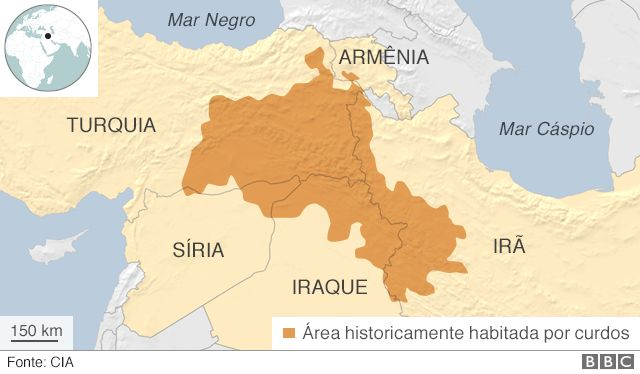
\includegraphics[width=1.02326in,height=0.57564in]{media/image1.jpeg}\textgreater{}

Hoje sabemos que o átomo é formando pelo núcleo (contendo prótons e
nêutrons) e pela eletrosfera (contendo elétrons). Sabemos ainda que um
conjunto de átomos com mesma propriedade constitui um elemento químico,
de forma que em conjunto podem formar substâncias. Estas substâncias
podem ser simples ou compostas. Juntas, duas ou mais substâncias formam
misturas, que podem ser homogêneas ou heterogêneas.

Na natureza a matéria pode ser encontrada em três estados físicos:
sólido, líquido ou gasoso. O que promove essa diferença é a organização
das moléculas, ou seja, a forma que os átomos que a compõem se organizam
e se movimentam. Há ainda a possibilidade de transitar entre os estados
da matéria por meio de mudanças na temperatura.

Os micro-ondas, por exemplo, são utensílios que promovem a transferência
de calor e mudança no estado físico, através da agitação das moléculas
de água presentes no alimento por meio de ondas eletromagnéticas. Essas
ondas se propagam sem meios materiais, assim como o wi-fi e a luz.
Existem ainda as ondas mecânicas, que necessitam de meios materiais,
como o som. As ondas podem ser classificadas de acordo com a direção da
sua propagação (podendo ser uni, bi ou tridimensional) e direção da
vibração (podendo ser longitudinal ou transversal).}

\colorsec{Atividades}

\num{1}  Leia as seguintes afirmações e aponte com V as verdadeiras e F as falsas:

\begin{boxlist}
\item Luz, som e calor constituídos de matéria \alternativa{F -- Luz, som e calor são
formas de energia e não de matéria}

\item Matéria é tudo aquilo que tem massa e ocupa lugar no espaço \alternativa{V}

\item A energia pode ser criada a partir da matéria \alternativa{F -- A energia não
se cria e nem se destrói, apenas se transforma}

\item Energia e matéria não podem sofrer transformações \alternativa{F -- Tanto
energia quanto matéria sofrem transformações}
\end{boxlist}

\coment{A questão avalia a capacidade do aluno de identificar afirmações falsas
sobre os conceitos de matéria e energia. Professor, atenção ao explicar
o conceito de matéria já que para a física moderna existem diferentes
tipos de matéria no Universo.}

\num{2}  De acordo com as transformações que a matéria pode sofrer coloque F
  para as transformações físicas e Q para as transformações químicas:

\begin{boxlist}
\item Amassar um papel \alternativa{(F)}

\item Queimar madeira \alternativa{(Q)}

\item Ferver água \alternativa{(F)}

\item Formação de ferrugem \alternativa{(Q)}

\item Misturar água com sal \alternativa{(F)}

\item Apodrecimento do tomate \alternativa{(Q)}
\end{boxlist}

\coment{Habilidade BNCC: (EF09CI01) Investigar as mudanças de estado físico da
matéria e explicar essas transformações com base no modelo de
constituição submicroscópica. A questão avalia a capacidade do aluno de
diferenciar transformações químicas e físicas da matéria. Professor,
justificar cada uma das frases a partir do conceito de transformação
química e física.}

\num{3} Escreva em ordem cronológica quais os modelos atômicos propostos pelos cientistas: Dalton, Thomson, Rutherford-Bohr. Apontando características principais sobre cada um deles.

\linhas{8}

\coment{Habilidade BNCC: (EF09CI03) Identificar modelos que descrevem a
estrutura da matéria (constituição do átomo e composição de moléculas
simples) e reconhecer sua evolução histórica. Espera-se que os alunos
descrevam o modelo de Dalton ``bola de bilhar'' descrevendo o átomo como
uma esfera maciça e indivisível, o modelo de Thomson ``pudim de passas''
e a presença de partículas subatômicas carregadas e estáticas, o modelo
de Rutherford-Bohr ``sistema solar'' que descreve o átomo como uma
estrutura formada por uma junção de partículas carregadas positivamente
no centro, chamado de núcleo e partículas com carga negativa orbitando
ao redor do núcleo formando a eletrosfera. Professor, estimule os alunos
a pensarem sobre a evolução do conhecimento científico.}

\num{4}  Observe a imagem e indique o nome correto, o local e sua respectiva
  carga para cada uma das partes do átomo:

%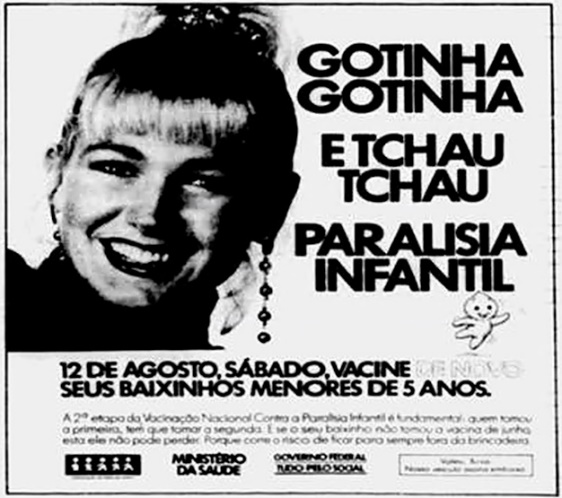
\includegraphics[width=2.02609in,height=1.43070in]{media/image2.jpeg}

%Fonte: Representação do átomo. Disponível em: \url{https://pixabay.com/pt/illustrations/átomo-símbolo-personagem-resumo-68866/}. Acessado em: 15 de fevereiro de 2023.

\linhas{5}

\coment{Habilidade BNCC: (EF09CI03) Identificar modelos que descrevem a
estrutura da matéria (constituição do átomo e composição de moléculas
simples) e reconhecer sua evolução histórica. Espera-se que o aluno
identifique os elétrons (esferas cinzas), presentes na eletrosfera com
carga negativa. Os prótons (esferas vermelhas), no núcleo com carga
positiva. Os nêutrons (esferas azuis), também presentes no núcleo com
carga neutra.}

\num{5} Joana observava sua tia fazer um café, e notou que à medida que a temperatura na chaleira esquentava mais fumaça era liberada pela própria chaleira. Joana então identificou que a molécula de água quando exposta ao calor muda suas características. A partir do seu conhecimento sobre moléculas e transformações físicas, avalie se a afirmação de Joana está correta e justifique.
  
\linhas{5}

\coment{Habilidade BNCC: (EF09CI01) Investigar as mudanças de estado físico da
matéria e explicar essas transformações com base no modelo de
constituição submicroscópica. Espera-se que os alunos identifiquem que a
afirmação de Joana está correta e expliquem que o estado físico da água
na chaleira muda à medida que o calor provoca agitação das moléculas de
água.}

\num{6} Dentre as misturas citadas a
  seguir diga quais são misturas HOMOGÊNEAS e HETEROGÊNEAS, no caso das
  misturas heterogêneas citar o número de fases:

\begin{escolha}
\item
  ÁGUA + SAL: \alternativa{homogênea}
\item
  ÁGUA + AREIA: \alternativa{heterogênea - duas fases}
\item
  AR ATMOSFÉRICO: \alternativa{homogênea}
\item
  ÁGUA + ÓLEO: \alternativa{heterogênea -- duas fases}
\item
  VINAGRE: \alternativa{homogênea}
\item
  GRANITO: \alternativa{heterogênea -- polifásica}
\end{escolha}

\coment{Habilidade BNCC: (EF09CI02) Comparar quantidades de reagentes e produtos
envolvidos em transformações químicas, estabelecendo a proporção entre
as suas massas. A questão avalia a capacidade do aluno de diferenciar
substâncias homogêneas de heterogêneas e identificar o número de fases
presentes nelas. Professor, citar a composição do Ar atmosférico,
vinagre e granito para ficar mais claro que tratam-se de misturas.}

\num{7}  A energia não pode ser criada ou destruída, apenas transformada. Essa
  afirmação da origem a imensas possibilidades de transformação no nosso
  cotidiano. Observe ao seu redor e cite pelo menos três exemplos onde
  você consegue observar transformação de energia.

\linhas{5}

\coment{Espera-se que o aluno cite exemplos de transformação de energia
presentes no seu cotidiano como a transformação de energia elétrica em
energia mecânica no funcionamento do ventilador, ou energia química em
energia em energia mecânica. Professor, estimule os alunos a pensarem em
diferentes exemplos de transformação de energia em seu cotidiano sempre
dando ênfase a conservação da energia.}

\num{8} A energia pode ter diversas fontes e inúmeras formas de ser utilizada. Pensando sobre as fontes RENOVÁVEIS e NÃO RENOVÁVEIS da energia marque com um X as fontes de energia RENOVÁVEIS:

\begin{boxlist}
\item Energia Solar \alternativa{X}

\item Energia Nuclear

\item Energia Eólica \alternativa{X}

\item Energia Hidráulica \alternativa{X}

\item Energia Fóssil
\end{boxlist}

\coment{A questão aborda da habilidade do aluno de identificar dentre as fontes
de energia aquelas que são renováveis, ou seja, possuem uma fonte
ilimitada e menos prejudicial ao meio ambiente durante sua obtenção e
consumo. Professor, lembre-se de ressaltar que mesmo energias renováveis
podem acarretar em danos ambientais e que se deve sempre ter mais de uma
fonte de energia para que não se sature um ambiente ou ecossistema.}

\num{9} A transmissão de imagem e som são essenciais para a comunicação nos
  dias atuais e por trás dessa transmissão existe muita física. É
  através do conceito de ondas que os engenheiros elaboram novas formas
  de nos comunicarmos. Sobre os tipos de ondas marque V para verdadeiro
  e F para falso:

\begin{boxlist}
\item Ondas eletromagnéticas necessitam do meio para se propagar \alternativa{(F) --
Ondas eletromagnéticas se propagam no vácuo}

\item Ondas sonoras são um exemplo de ondas longitudinais \alternativa{(V)}

\item Ondas mecânicas se propagam no vácuo \alternativa{(F) -- Ondas mecânicas
necessitam do meio para se propagar}

\item Ondas podem ser unidimensionais, bidimensionais e tridimensionais \alternativa{(V)}
\end{boxlist}

\coment{Habilidade BNCC: (EF09CI06) (EF09CI06) Classificar as radiações
eletromagnéticas por suas frequências, fontes e aplicações, discutindo e
avaliando as implicações de seu uso em controle remoto, telefone
celular, raio X, forno de micro-ondas, fotocélulas etc. A questão avalia
a habilidade dos alunos de identificar falsas premissas em relação aos
tipos de ondas.}

\num{10} Observe a imagem e responda:

%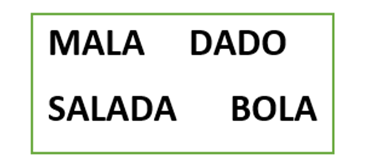
\includegraphics[width=2.91389in,height=1.47847in]{media/image3.png}

\begin{escolha}
\item  Que tipo de fenômeno pode ser observado na imagem?

\linhas{1}

\coment{Refração}

\item Que tipo de onda está relacionada com a propagação da luz?

\linhas{1}

\coment{Ondas eletromagnéticas}

\item Cite um exemplo onde esse conhecimento sobre a propagação da luz é utilizado no seu cotidiano?

\linhas{1}

\coment{Câmera fotográfica, televisão, cinema, etc.}
\end{escolha}

\coment{Habilidade BNCC: (EF09CI06)
Classificar as radiações eletromagnéticas por suas frequências, fontes e
aplicações, discutindo e avaliando as implicações de seu uso em controle
remoto, telefone celular, raio X, forno de micro-ondas, fotocélulas etc.
A questão avalia a habilidade dos alunos a capacidade de relacionar os
seus conhecimentos sobre a transmissão da luz visível e suas
consequências para a formação de imagens, como é o caso das câmeras
fotográficas, televisões e celulares por exemplo.}

\num{11} O uso de aplicativos de mensagens foi essencial para a comunicação no período de pandemia. Com base nos seus conhecimentos de ondas eletromagnéticas explique como é possível enviar uma imagem pelo celular para uma pessoa que se encontra em outra cidade.


\linhas{3}

%\textless{}Diagramação, por favor, baixar a imagem do banco presente no seguinte link (\url{https://pixabay.com/pt/vectors/interface-whatsapp-apps-andróide-1660652/}) e fazer o corte, deixando apenas a imagem do meio, conforme referência:

\coment{Espera-se que os alunos descrevam que através de ondas eletromagnéticas,
a mensagem enviada é transferida do emissor ao receptor, e as
frequências de onda que formam a imagem são reproduzidas no celular de
quem recebeu a foto. Professor, aqui é necessário se ater apenas ao
conceito básico de transmissão de informação por ondas eletromagnéticas
em especifico a transmissão de imagem. Já que esse processo é muito mais
complexo do que o conjunto de conhecimentos trabalhados até aqui. Pode
ser sugerido que os alunos pesquisem em casa sobre esse processo e como
funciona a tecnologia WI-FI.

Habilidade BNCC: (EF09CI06) Classificar as radiações eletromagnéticas
por suas frequências, fontes e aplicações, discutindo e avaliando as
implicações de seu uso em controle remoto, telefone celular, raio X,
forno de micro-ondas, fotocélulas etc. A questão avalia a habilidade dos
alunos de interpretar e relacionar acontecimentos do seu cotidiano com
conceitos físicos complexos.}

\colorsec{SEÇÃO TREINO}

\num{1}

\begin{quote}
``A The Ocean Cleanup é uma ONG que pretende acabar com a Grande
Mancha do Pacífico, a imensa ilha de plástico que flutua no maior dos
oceanos, usando um sistema que captura o lixo, que depois será
retirado por um navio. O sistema funciona com uma grande barreira
flutuante e uma tela que fica submersa a uma profundidade de 3 metros,
e pode capturar o lixo que não está boiando na superfície.''

\fonte{The Ocean Cleanup: sistema de barreiras flutuantes quer tirar plástico
do Pacífico. Disponível em:
https://meiobit.com/390064/the-cleanup-ocean-limpar-plastico-do-pacifico/.
Acesso: 17 de fevereiro 2023.}
\end{quote}

A ideia de catar o lixo boiando sobre a água que será barrada pelas
barreiras desenvolvidas pela ONG só é possível graças a propriedade da
matéria:

\begin{escolha}
\item Volume

\item Maleabilidade

\item Brilho

\item Densidade
\end{escolha}

\coment{Fácil -- Habilidade BNCC: (EF09CI01) Investigar as mudanças de estado
físico da matéria e explicar essas transformações com base no modelo de
constituição submicroscópica.

a) INCORRETA, pois, a matéria com um todo possui volume, dessa forma essa
  propriedade não justifica o fato de o lixo flutuar na superfície da
  água. Um exemplo é a areia que possui volume, mas sedimenta e é
  encontrada no fundo do mar.

b) INCORRETA, pois, a maleabilidade refere-se à capacidade da matéria ser
  moldada, o que não é a propriedade que faz com que esse lixo possa ser
  catado pelos membros da ONG.

c) INCORRETA, pois, o brilho não é uma propriedade relevante para que o
  lixo seja catado na superfície da água, já que ele não influencia
  diretamente na densidade do material.

d) CORRETA, pois, é graças a diferença de densidade do lixo e da água que
  esses resíduos boiam na superfície e podem ser catados pelos membros
  da ONG.}

\num{2}

\begin{quote}
Pesquisadores descrevem movimento de elétrons que levam à aurora
pulsante, evento multicolorido e brilhante na magnetosfera. O que os
cientistas conseguiram observar foi uma evidência direta da origem da
aurora pulsante: uma verdadeira chuva de elétrons envolvida em ondas
de plasma (estado físico da matéria similar ao gás, mas com partículas
ionizadas).

\fonte{Adaptado de Cientistas observam 'chuva de elétrons' que dá origem a
fenômeno brilhante no céu; veja vídeo. G1 Ciência e Saúde. 2018.
Disponível em:
https://g1.globo.com/ciencia-e-saude/noticia/cientistas-observam-chuva-de-eletrons-que-da-origem-a-fenomeno-brilhante-no-ceu-veja-video.ghtml.
Acesso: 19 de fevereiro 2023.}
\end{quote}

Quais características do elétron fazem com que eventos como a aurora
pulsante seja possível?

\begin{escolha}
\item
  Elétrons encontram-se no núcleo do átomo e liberam energia mudando
  entre as camadas de valência
\item
  Elétrons são partículas neutras que transferem cargas elétricas ao se
  movimentarem pela eletrosfera
\item
  Elétrons são partículas de carga negativa que se encontram na
  eletrosfera, capazes de se movimentar liberando energia
\item
  Elétrons possuem cargas negativas, presas ao núcleo que quando se
  movimentam liberam energia
\end{escolha}

\coment{Média -- Habilidade BNCC: (EF09CI03) Identificar modelos que descrevem a
estrutura da matéria (constituição do átomo e composição de moléculas
simples) e reconhecer sua evolução histórica.

a) INCORRETA, pois os elétrons não se encontram no núcleo atômico.

b) INCORRETA, pois os elétrons são partículas que apresentam cargas
  negativas.

c) CORRETA, pois elétrons de fato são partículas negativas que se
  encontram na eletrosfera capazes de se movimentar e liberar energia.

d) INCORRETA, pois os elétrons são ficam presos ao núcleo, e sim livres
  na eletrosfera.}

\num{3}

\begin{quote}  
Você tem a sensação de que o sinal de Wi-Fi fica mais fraco no
banheiro do que em outros cômodos? Saiba que isso não é um mito e
existe uma explicação para isso. Os grandes vilões do Wi-Fi no
banheiro são os espelhos. Quanto maior seu tamanho, maior é a chance
de ele interferir no sinal da Internet. Isso porque, por trás do
vidro, há uma camada de metal, responsável por refletir a luz.

\fonte{Entenda por que o sinal da Internet Wi-Fi é mais lento no banheiro. G1
Techtudo. 03/11/2018. Disponível em:
https://www.techtudo.com.br/listas/2018/11/entenda-por-que-o-sinal-da-internet-wi-fi-e-mais-lento-no-banheiro.ghtml.
Acesso em: 19 de fevereiro de 2023.}
\end{quote}

Com base nas informações do texto e em seus conhecimentos, justifique a
relação da presença de espelhos no banheiro com a baixa qualidade de
sinal de Wi-Fi nesse ambiente.

\begin{escolha}
\item
  O sinal do Wi-Fi é transmitido através de ondas eletromagnéticas que
  são capturadas pelo metal que é bom condutor de energia, atrapalhando
  a transmissão.
\item
  A transmissão Wi-Fi acontece por meio de ondas mecânicas, dessa forma
  estruturas sólidas com potencial de reflexão, como os espelhos,
  atrapalham a transmissão.
\item
  A camada de metal reflete sinal de Wi-Fi, evitando que ele se
  propague, já que se trata de ondas eletromagnéticas, que necessitam de
  objetos para se propagar no meio.
\item
  O sinal do Wi-Fi é transmitido através dos mesmos princípios que o som
  e sua propagação dependem de meios opacos para acontecer, o brilho do
  espelho dificulta a transmissão.
\end{escolha}

\coment{Difícil -- Habilidade BNCC: (EF09CI06) Classificar as radiações
eletromagnéticas por suas frequências, fontes e aplicações, discutindo e
avaliando as implicações de seu uso em controle remoto, telefone
celular, raio X, forno de micro-ondas, fotocélulas etc.

a) CORRETA, pois de fato a transmissão Wi-Fi ocorre por meio de ondas
  eletromagnéticas que são capturadas por materiais que possuem boa
  capacidade elétrica como é o caso do metal, presente nos espelhos.

b) INCORRETA, pois a transmissão do sinal Wi-Fi não ocorre por meio de
  ondas mecânicas, e sim por meio de ondas eletromagnéticas.

c) INCORRETA, pois por se tratar de uma propagação através de ondas
  eletromagnéticas, o Wi-Fi é capaz de se propagar no vacúo.

d) INCORRETA, pois o sinal Wi-Fi não é transmitido através do mesmo tipo
  de onda que o som, já que o Wi-Fi é transmitido através de ondas
  eletromagnéticas e o som através de ondas mecânicas.}

\chapter{2. Vida e evolução}

\coment{Durante a explicação das teorias evolucionista, recomendamos que você
utilize a lousa como recurso para deixar claro as ideias antagonicas
existentes nas teorias de Lamarck e Darwin. Além disso, é importante
ressaltar que as ideias de Lamarck, apesar de não aplicadas hoje, foram
importante para que estudiosos da época pudesse basear seus estudos,
assim você mostra aos alunos que a ciência é construída ``de passo em
passo'' e em conjunto. Durante a explicação sobre classificação
biológica, lembre-se de ressaltar que reino é a categoria mais
abrangente, enquanto espécie é a categoria mais específica, e é
importante comentar que os nomes estejam em latim e que o nome da
espécie e do gênero sejam destacados. Para finalizar a aula, converse
com os estudantes sobre a diversidade de espécies presentes em nosso
país e proponha que em grupo elaborem propostas de intervenção que
possam conter o avanço do desmatamento em nosso país.}

\conteudo{Hoje conhecemos cerca de 1,5 milhão de espécies presentes em nosso
planeta. Mas as estimativas vão além, dizem que existem cerca de 10 a 50
milhões de seres vivos que ainda não foram classificados! Cada uma
dessas espécies possui características individuais e modo singular de
interagir com o meio biótico (conjunto de seres vivos, como fauna e
flora) e abiótico (conjunto de seres não vivos, como água e luz). Mas
como pode haver uma diversidade tão imensa de seres vivos?

Há muito tempo, estudiosos se fizeram essa mesma pergunta, a partir dela
começaram a cunhar as teorias evolucionistas, que afirmam que os seres
vivos mudam ao longo do tempo. Lamarck acreditava que os seres vivos
mudariam para se adaptar em um ambiente e essas novas características
adquiridas seriam repassadas. Já Darwin, afirmou que as mudanças
existente entre as espécies eram decorrentes da seleção natural, ou
seja, os seres vivos mais aptos seriam selecionados pelo ambiente,
sobrevivendo poderiam se reproduzir e repassar seus caracteres.

Hoje
sabemos que a evolução das espécies é um processo constante, atemporal,
acontece há milhões de anos e atua sobre todos os organismos vivos
selecionando as espécies que se adaptam ás mudanças ambientais. Diante
disso, nos deparamos com outra questão: como organizar tantos seres? Na
biologia, temos organizações hierarquicas, nas quais podemos organizar a
vida desde átomos, célula e sistemas (como o respiratório, endócrino,
muscular) até ecossistemas e biosfera, conforme a figura a seguir:

%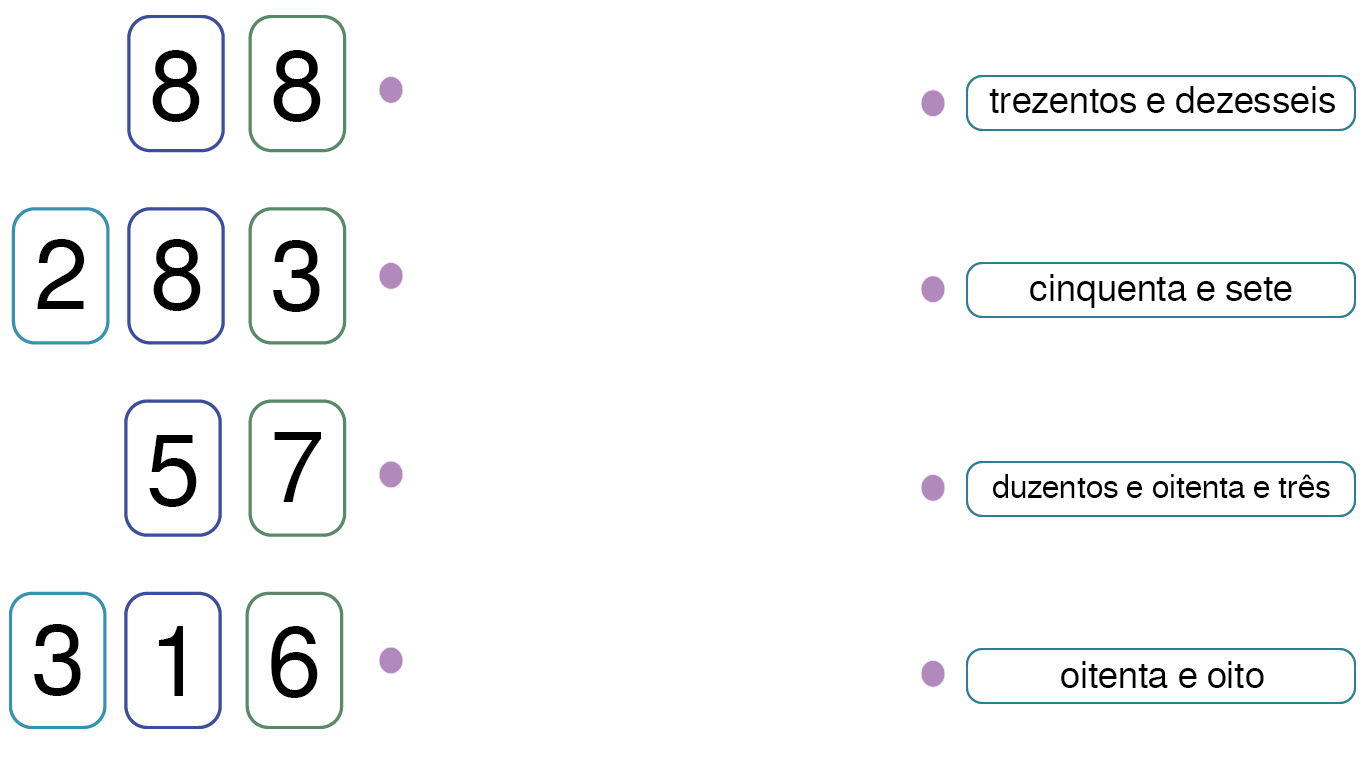
\includegraphics[width=1.71875in,height=1.66389in]{media/image5.png}
%\textless{}Diagramação, por favor, baixar imagem presente no link e
%traduzir legenda.
%\url{https://www.dreamstime.com/royalty-free-stock-images-living-world-image23729369}
%Se não for possível baixar, por favor vetorizar esquema semelhante.
%\textgreater{}

Ou podemos seguir de uma maneira mais específica, organizando as
espécies que existem no planeta por meio da classificação biológica.
Essa tarefa é tão extensa que existe uma área específica dedicada a
identificar, nomear e classificar os seres vivos: a taxonomia. Veja a
seguir os níveis de organização taxonômicos da espécie humana.

Nossa espécie é uma das que mais se prolifera no mundo, ao passo que
também é uma das que mais o destrói. No Brasil, dos seus seis biomas
(Amazônia, Caatinga, Cerrado, Pantanal, Mata Atlântica e Pampa), todos
já tem uma porcentagem destruída. Sendo o desmatamento da Amazônia um
dos mais graves. Além do desequilíbrio ambiental provocado pela perda da
vegetação nativa, há ainda a problemática do aumento da transmissão de
doenças, tendo em vista que animais silvestres perdem seu habitat e
passam a viver mais próximos da população humana, podendo disseminar
doençar. Um exemplo é a COVID-19, acredita-se que a zoonose estava
presente em morcegos e acabou alcançando a espécie humana devido a caça
desses animais. Portanto, é evidente que tanto o meio ambiente depende
de nós quanto nós dependemos dele para coexistirmos. E, como ferramenta
aliada nesse processo de conservação das espécis, vale destacar as
unidades de conservação.}

\num{1} Jean-Baptiste de Lamarck foi um naturalista francês assim como Charles
  Darwin. Ambos se interessaram por um mesmo processo: a evolução das
  espécies. A partir de suas observações, cada um deles elaborou teorias
  que explicassem esse processo. Sabendo disso, responda:

\begin{escolha}
\item No que consiste a teoria de cada um deles?

\linhas{7}

\coment{Habilidade BNCC - EF09CI10 Comparar as ideias evolucionistas de Lamarck
e Darwin apresentadas em textos científicos e históricos, identificando
semelhanças e diferenças entre essas ideias e sua importância para
explicar a diversidade biológica.

Lamarck acreditava que os seres vivos poderiam mudar espontaneamente
para se adaptar ao ambiente, girafas por exemplo, ao fortalecer o
pescoço poderiam acabar fazendo-o crescer e, ao reproduzir, passariam
essa características a seus descendentes. Darwin acreditava que os seres
vivos mais aptos a um determinado ambiente passariam por um processo de
seleção natural, por exemplo, girafas de pescoço mais longo seriam
privilegiadas por conseguirem se alimentar mais facilmente e
sobreviveriam no ambiente, enquanto as de pescoço curto enfretariam mais
desafios para conseguir se alimentar e poderiam acabar morrendo sem
passar seus genes adiante.}

\item Apesar das diferenças, os estudiosos possuíam pontos em comum que uniam suas teorias. Quais eram?

\linhas{4}

\coment{Habilidade BNCC - EF09CI08 Associar os gametas à transmissão das
características hereditárias, estabelecendo relações entre ancestrais e
descendentes.

Ambos acreditavam que as espécies se modificavam com o tempo, que as
características eram passadas para seus descendentes, e que essas
características eram influenciadas de alguma forma pelo ambiente.}
\end{escolha}

\num{2} Quando se fala em biodiversidade, costuma-se pensar no verde das florestas. Mas é no azul dos oceanos que está a última fronteira da vida e a maior diversidade de espécies do planeta. Por exemplo, robôs a serviço do censo descobriram sob o gelo do Ártico uma cadeia vulcânica coberta por micro-organismos. Um satélite localizou uma aglomeração de centenas de tubarões no meio do Pacífico Norte. Fontes quentes em águas gélidas são o lar de peixes bizarros e vermes gigantes. Até a década passada, o homem conhecia cerca de 230 mil espécies marinhas. Esse contingente saltou para quase 236 mil. E estima-se que o número real ultrapasse um milhão, pelo menos. Juntos, os 17 projetos do Censo exploraram 5\% dos oceanos.

\fonte{Referência: Oceanos abrigam a maior diversidade da Terra.
https://oglobo.globo.com/saude/ciencia/oceanos-abrigam-maior-diversidade-da-terra-3036406.
Acesso em: 23/02/2023.}

O que explica a grande diversidade encontrada por esses pesquisadores
durante sua exploração no oceano?

\linhas{4}

\coment{Tendo em vista que o oceano é um ambiente extenso e diverso, pode-se
afirmar que ao longo da evolução das espécies marinhas elas foram
selecionadas para conseguir sobreviver em cada um desses ambientes, o
que gerou a alta diversidade de espécies existentes no oceano.}

\num{3}  O exemplo clássico da hipótese de Lamarck é o das girafas, que depois ficou conhecida como "lamarquismo": os animais teriam herdado o pescoço longo de seus antepassados, e essa característica foi se aprofundando para permitir alcançar os ramos mais altos das árvores, de cujas folhas elas se alimentam.

Mas em 1859, a hipótese de Lamarck foi ofuscada quando Charles Darwin
lançou o livro A Origem das Espécies. Na obra, o britânico descreve como
os traços de cada espécie viva surgem ao longo de várias gerações,
conforme mutações genéticas benéficas são selecionadas pelo ambiente.
Hoje, a teoria da Evolução de Charles Darwin é considerada um fato
científico.

\fonte{Referência: Como uma aldeia no Ártico ajudou a ampliarmos o que sabemos
sobre Evolução. \url{https://www.bbc.com/portuguese/geral-42420424}.
Acesso em 23/02/2023. Adaptado.}

Apesar da ideia de Lamarck não ser aplicada hoje, ela foi importante
para os estudiosos da época. Explique o porquê.

\linhas{6}

\coment{Habilidade BNCC - EF09CI10 Comparar as ideias evolucionistas de Lamarck
e Darwin apresentadas em textos científicos e históricos, identificando
semelhanças e diferenças entre essas ideias e sua importância para
explicar a diversidade biológica.

Lamarck teve ideias revolucionárias para seu tempo ao refletir sobre a
influência do meio ambiente sobre os organismos. Apesar de não ter
formulado a teoria que utilizamos hoje (evolução por meio da seleção
natural), suas ideias estabeleceram as bases para que, posteriormente,
estudiosos pudessem refletir mais sobre o cenário exposto por ele e
elaborar o conceito que adotamos hoje.}

\num{4}  Sobre os níveis de organização em biologia, marque V ou F:

\begin{boxlist}
\item A organização começa no átomo. \alternativa{(V)}

\item A célula é a unidade básica da vida. \alternativa{(V)}

\item A nível mais alto e complexo é o organismo. \alternativa{(F)}

\item Um conjunto de ecossistemas formam uma comunidade. \alternativa{(F)}
\end{boxlist}

\num{5}  O corpo humano é complexo, formado por \preencher
  que trabalham em sintonia para que o organismo funcione da melhor
  forma possível e que a sobrevivência do indivíduo seja garantida.

\fonte{Referências: Físicos investigam interações.
https://jornal.usp.br/ciencias/ciencias-exatas-e-da-terra/fisicos-investigam-interacoes-entre-sistemas-do-corpo/
. Acesso em 23/02/2023.}

Qual nível de organização biológica melhor preenche a lacuna do texto?
Cite alguns exemplos do agrupamento citado.

\coment{Sistemas. Sistema respiratório, nervoso, esquelético, reprodutor.}

\num{6}  Escreva, em ordem hierárquica, os níveis de organização biológica existentes.

\linhas{2}

\coment{Átomo, mólecula, organela, célula, tecido, órgão, sistema, organismo,
população, comunidade, ecossistema, bioma, biosfera.}

\num{7}

\begin{quote}
\textbf{Seres vivos ganham nova classificação após 285 anos.}

O universo científico criou uma nova forma de classificar os organismos
vivos 285 anos após a invenção do Systema Naturae pelo botânico sueco
Carlos Lineu. A nova proposta, publicada nos livros PhyloCode e
Phylonym, leva em consideração a Teoria da Evolução de Charles Darwin e
foi organizada por cerca de 200 especialistas. Entre os responsáveis
pela nova classificação, o professor Max Cardoso Langer, do Departamento
de Biologia, da Faculdade de Filosofia, Ciências e Letras de Ribeirão
Preto (FFCLRP) da USP, explica que a modificação foi necessária porque a
invenção de Lineu é anterior à teoria de Darwin e, naquela época,
classificou os organismos pelas características anatômicas. Lineu não
sabia que ``os organismos mudam morfologicamente ao longo do tempo'',
mas, apesar disso, ``o sistema de denominação permanece sendo como o
daquela época''. Para o novo sistema, cientistas buscaram por linhagens
evolutivas dos seres para então defini-los. ``Ao invés de definir as
aves como os animais que têm penas, podemos definir, por exemplo,
colocando todas as aves viventes em uma árvore filogenética e descer a
linha de ancestralidade até chegar a um único ancestral comum. Todas as
espécies que descendem desse ancestral comum serão chamadas aves.''

\fonte{Referência: Seres vivos ganham nova classificação após 285 anos.
https://jornal.usp.br/ciencias/seres-vivos-ganham-nova-classificacao-apos-285-anos/
. Acesso em 23/02/2023.}
\end{quote}

A qual área da biologia o texto está se referindo?

\linhas{2}

\coment{Taxonomia, ramo responsável por descrever, identificar e nomear os seres
vivos de acordo com critérios de classificação.}

\num{8}  Acerca do padrão de nomenclatura biológica das espécies, marque V ou F.

\begin{boxlist}
\item homo sapiens é a forma correta de escrita da espécie humana. \alternativa{(F)
Pois os critérios de nomeclatura exigem que o nome da espécie seja
destacado e o primeiro nome inicie com letra maiúscula.}

\item A nomeclatura científica é, obrigatoriamente, binomial. \alternativa{(V)}

\item O primeiro nome é chamado de epíteto específico e o segundo de
epíteto generico. \alternativa{(F) Pois o primeiro nome se refere ao gênero da
espécie, enquanto o segundo, a especifíca, por isso é nomeado de epíteto
específico.}

\item O latim foi escolhido para nomear espécies por ser uma língua bonita
e culta. \alternativa{(F) Pois o latim foi escolhido por ser uma língua morta, sendo
assim, a língua não evolui, ou seja não existem modificações no
vocabulário.}

\item \emph{Trichechus manatus} e \emph{Trichechus inunguis} são duas
espécies pertencentes a um mesmo genero. \alternativa{(V)}

\item As regras de nomeclatura científica permitem que cientistas de
qualquer local do mundo possam compartilhar informações sobre as
espécies existentes. \alternativa{(V)}
\end{boxlist}

\num{9}  A seguir você encontra todas as categorias taxonômicas existentes.

\begin{quote}
GÊNERO -- CLASSE -- FILO -- ESPÉCIE -- FAMÍLIA -- ORDEM -- REINO
\end{quote}

Ordene-as de maneira hierárquica, da mais abrangente à mais específica.

\linhas{2}

\coment{Reino -- Filo -- Classe -- Ordem -- Família -- Gênero -- Espécie}

\num{10}  Sobre as categorias taxonômicas, marque V ou F

\begin{boxlist}
\item Família é a categoria mais abrangente. \alternativa{(F) A categoria mais
abrangente é o domínio.}

\item Espécie é a categoria mais específica. \alternativa{(V)}

\item Ornitorrincos e seres humanos, apesar de bem diferentes, ocupam a
mesma classe por serem mamíferos. \alternativa{(V)}

\item Existem seis reinos distintos: animalia, plantae, fungi, monera,
protista e vírus. \alternativa{(F) Existem cinco reinos: animalia, plantae, fungi,
monera e protista. Vírus não são considerados seres vivos e por isso não
entram em nenhuma categoria taxonomica.}
\end{boxlist}

\num{11}  Bioma exclusivamente brasileiro e responsável por abrigar o Semiárido
  e ocupa cerca de 11\% do território nacional e 54\% da Região
  Nordeste. O representante do Centro de Assessoria e Apoio aos
  Trabalhadores e Instituições Não Governamentais Alternativas, Paulo
  Pedro de Carvalho, advertiu que esse foi o bioma que mais sofreu
  degradação com as mudanças climáticas.

\fonte{Referência:
https://www12.senado.leg.br/noticias/materias/2022/04/27/audiencia-destaca-riqueza-da-caatinga-e-alerta-para-efeitos-das-mudancas-climaticas-no-bioma
. Acesso: 23/02/2023.}

\begin{escolha}
\item A qual bioma o texto se refere?

\linhas{1}

\coment{Caatinga}

\item Quais os outros biomas que o nosso país abriga?

\linhas{1}

\coment{Cerrado, Pampa, Mata Atlântica, Amazônia, Pantanal.}
\end{escolha}

\num{12}  Sobre conservação da biodiversidade, marque V ou F

\begin{boxlist}
\item Unidade de conservação é uma área que engloba tanto espaço
territorial quanto recursos naturais, tendo como objetivo a conservação
da fauna e flora de uma região. \alternativa{(V)}

\item A contaminação da água, solo e ar, assim como a destruição de
habitat e o uso sustentável de recursos são ameaças para a
biodiversidade. 
\alternativa{(F) O uso sustentável dos recursos é uma das estratégias que devem ser adotadas para a preservação da biodiversidade.}

\item As unidades de conservação de proteção integral tem como objetivo
manter a natureza livre da interferência humana, enquanto a de uso
sustentável preza pela conciliação entre conservação e uso sustentável
de recursos. \alternativa{(V)}

\item Biodiversidade é um termo que descreve a riqueza de espécies
existentes no planeta, incluindo plantas, animais, fungos e
microorganismos. A conservação e sobrevivência desses seres está
intimamente ligada a sobreviência da espécie humana. \alternativa{(V)}
\end{boxlist}

\coment{Habilidade BNCC - EF09CI12 Justificar a importância das unidades de
conservação para a preservação da biodiversidade e do patrimônio
nacional, considerando os diferentes tipos de unidades (parques,
reservas e florestas nacionais), as populações humanas e as atividades a
eles relacionados.}

\colorsec{SEÇÃO TREINO}

\num{1}  Mais de 21 anos após o anúncio do descobrimento da sequência genética
  dos humanos, a coalizão do Projeto do Genoma Humano publicou um artigo
  científico que estabelece o primeiro mapa genético totalmente completo
  da espécie humana. Até 2021, cerca de 92\% do código genético humano
  era conhecido. Segundo os autores do estudo, publicado na revista
  científica Science, as novas informações trazem dados importantes
  sobre doenças e características evolutivas da raça humana.

\fonte{Referência: https://agenciabrasil.ebc.com.br/saude/noticia/2022-03/cientistas-publicam-artigo-que-conclui-mapeamento-genetico-humano. Acesso em 23/02/2023.}

A investigação das características citadas é possível graças à:

\begin{escolha}
\item
  Hereditariedade.
\item
  Paleontologia.
\item
  Conservação.
\item
  Taxonomia.
\end{escolha}

\coment{Fácil -- Habilidade BNCC (EF09CI08) Associar os gametas à transmissão
das características hereditárias, estabelecendo relações entre
ancestrais e descendentes.

a) CORRETA, pois a hereditariedade trata das características e
  informações genéticas transmitidas a cada geração. Ao estudar o código
  genético para entender sobre doenças e outras características da raça
  humana as relações ancestrais-descendentes estão sendo
  desmistificadas.

b) INCORRETA, pois a paleontologia trata do estudo de seres vivos que
  habitaram a terra em um passado remoto.

c) INCORRETA, pois a conservação trata do estudo de técnicas alternativas
  que resultem no uso sustentável dos recursos e preservação das
  espécies.

d) INCORRETA, pois a taxonomia trata de descrever, identificar e nomear
  seres vivos a partir de critérios estabelecidos.}

\num{2}  Em um estudo recente, cientistas da França e Espanha, estudaram a
  coloração ornamental da ave chapim-azul (\emph{Cyanistes caeruleus}).
  O chapim-azul caracteriza-se por ter uma coloração bastante vistosa.
  Sua coroa azul e peito amarelo são marcantes. Os resultados mostram
  que em duas populações estudadas, as coroas azuis e os peitos amarelos
  são menos visíveis do que quando o estudo começou. Além disso, nos
  verões mais quentes e secos os chapim-azul apresentavam cores menos
  vistosas, tanto azul quanto amarela. Isso, juntamente ao aumento da
  temperatura e diminuição da precipitação na área de estudo, sugere que
  a redução da coloração nesta população é consequência das mudanças
  climáticas.

\fonte{Referência: https://www.bbc.com/portuguese/geral-62048972 . Adaptado.
Acesso em 23/02/2023.}

Qual teoria explica o fenômeno apresentado na pesquisa?

\begin{escolha}
\item
  Seleção natural, ao notar as mudanças ambientais, os pássaros se
  modificaram para que pudessem sobreviver.
\item
  Lamarckismo, ao notar as mudanças ambientais, os pássaros se
  modificaram para que pudessem sobreviver.
\item
  Seleção natural, a mudança ambiental exerce uma pressão sobre a
  espécie, selecionando apenas os mais aptos a sobrevivência.
\item
  Lamarckismo, a mudança ambiental exerce uma pressão sobre a espécie,
  selecionando apenas os mais aptos a sobrevivência.
\end{escolha}

\coment{Média -- Habilidade (EF09CI10) Comparar as ideias evolucionistas de
Lamarck e Darwin apresentadas em textos científicos e históricos,
identificando semelhanças e diferenças entre essas ideias e sua
importância para explicar a diversidade biológica.

a) INCORRETA, pois a alternativa descreve o conceito descrito por
  Lamarck, no qual os indivíduos se modificam para se adaptar ao
  ambiente. Seleção natural é um conceito próximo a ideia de Darwin, que
  menciona que o ambiente seleciona os indivíduos mais aptos,

b) INCORRETA, pois a alternativa descreve o conceito de Lamarck, que
  posteriormente foi estudado e modernizado por Darwin, dando origem a
  teoria que utilizamos hoje: a seleção natural.

c) CORRETA, pois as mudanças ambientais implicam em condições ambientais
  ruins, por exemplo, alimento escasso. Com isso, obter energia fica
  mais difícil e por consequência, o investimento de energia em
  ornamentos (como cores fortes) também diminui. Sendo assim, o ambiente
  seleciona apenas os pássaros capazes de sobreviver sob estas
  condições.

d) INCORRETA, pois o Lamarck não acredita que o ambiente selecionava as
  espécies, na verdade, sua teoria falava sobre a mudanças das espécies
  frente as imprevisibilidades do ambiente.}

\num{3}

\begin{quote}
\textbf{Idema propõe criação de nova unidade de conservação da caatinga no Rio
Grande do Norte}

"Refúgio da Vida Silvestre" será área de proteção do bioma e de
preservação das cabeceiras da bacia hidrográfica do Rio Potengi, segundo
órgão.

O Instituto de Desenvolvimento Sustentável e Meio Ambiente (Idema)
propôs a reserva de uma área para criação de uma unidade de conservação
da caatinga e das cabeceiras da bacia hidrográfica do Rio Potengi, no
Rio Grande do Norte.

\fonte{Referência:
https://g1.globo.com/rn/rio-grande-do-norte/noticia/2022/11/26/idema-propoe-criacao-de-nova-unidade-de-conservacao-da-caatinga-no-rio-grande-do-norte.ghtml
. 23/02/2023.}
\end{quote}

Qual alternativa indica uma possível justificativa para defender a criação da unidade de conservação citada?

\begin{escolha}
\item
  Devido à baixa riqueza de espécies na Caatinga, é necessário que hajam
  normas garantindo o isolamento geográfico desses indivíduos.
\item
  Devido à alta diversidade biológica endêmica e a extensão da Caatinga,
  é necessário que hajam normas garantindo a proteção adequada.
\item
  Devido à alta diversidade biológica e a extensão da Caatinga, é
  necessário criar medidas que favoreçam o comércio das espécies
  exóticas da região.
\item
  Devido à baixa riqueza de espécies na Caatinga, é necessário que hajam
  incentivos para a criação de indústria na área.
\end{escolha}

\coment{Média -- Habilidade (EF09CI12) Justificar a importância das unidades de
conservação para a preservação da biodiversidade e do patrimônio
nacional, considerando os diferentes tipos de unidades (parques,
reservas e florestas nacionais), as populações humanas e as atividades a
eles relacionados.

a) INCORRETA, pois a Caatinga é um bioma com um dos níveis de
  biodiversidade mais altos.

b) CORRETA, pois a Caatinga possui alta biodiversidade, a qual 15\% é
  endêmica, portanto, diante das mudanças ambientais, a construção de
  unidades de conservação nesse bioma deve ser priorizada para garantir
  a proteção adequada às espécies.

c) INCORRETA, pois o comércio de espécies exóticas é uma medida que iria
  prejudicar a biodiversidade presente na Caatinga, estando em posição
  antagonica ao objetivo das unidades de conservação.

d) INCORRETA, pois com a construção de indústrias o habitat de diversas
  espécies seria prejudicado, favorecendo a perda de biodiversidade e,
  portanto, estando em posição antagonica ao objetivo das unidades de
  conservação.}

\chapter{3. Terra e universo}

\coment{ORIENTAÇÕES PARA O PROFESSOR: Durante a explicação, acerca do surgimento
do universo, ressalte que o movimento da matéria não ocorreu somente no
momento do Big Bang. Reforce que o universo está em constante expansão
e, portanto, as galáxias estão se afastando. Se achar pertinente,
durante a explicação sobre o sistema solar, se aprofunde nas
características individuais de cada planeta, comentando, por exemplo,
sobre os anéis de Saturno. Para falar sobre a Terra, procure vincular
suas características ao dia a dia dos estudantes, para isso você pode
perguntar como os fenômenos comentados os impactam e qual a importância
da translação por exemplo, para o cotidiano deles.}

\conteudo{De onde viemos? Para responder temos que voltar bilhões de anos. Quando
toda a matéria e energia estava contida em um único ponto. Até que um
desequilíbrio provocou uma grande explosão chamada de ``Big Bang''.
Nesse segundo, toda a matéria se estendeu ao longo do espaço infinito.
Ao contrário do que podem pensar, esse processo de expansão continua e
continuará aumentando. Mas cientistas já levantaram a hipótese de uma
contração final, que fará tudo retornar ao ponto inicial, esse movimento
foi nomeado como ``Big Crunch''.

Mas afinal, onde estamos em meio a essa estrutura em expansão? Dentre as
milhares de galáxias existentes, fazemos parte da Via Láctea. Nela,
diversas estrelas nascem e morrem constantemente. E nós, estamos em um
sistema ao redor da estrela que chamamos de Sol. Nesse sistema estão
incluídos oito planetas: Mercúrio, Vênus, Terra e Marte (Esses planetas
são formados principalmente por rochas, por isso são chamados de
terrestres ou telúricos); Júpiter, Saturno, Urano e Netuno (Esses
planetas são formados principalmente por gases, por isso são chamados de
gasosos ou jovianos). Além deles, há ainda diversos satélites naturais
(como a nossa Lua), cometas, asteroides e outras partículas que vagam
por nossa galáxia. Por fim, é importante saber que Plutão (conhecido
como ``planeta anão'') é um corpo celeste presente em nosso sistema
solar que devido a uma decisão da União Astronômica Internacional deixou
de ser considerado planeta. Sendo o principal motivo o fato de plutão
não ter massa suficiente para limpar sua órbita de objetos menores.
Existem outros planetas anões como ele, sendo Ceres, Haumea, Makemake e
Éris.

%\textless{}Diagramação, por favor, baixar imagem presente no link
%(\url{https://br.freepik.com/vetores-gratis/sistema-solar-para-o-ensino-de-ciencias_24085043.htm\#query=sist%ema\%20solar\&position=5\&from_view=search\&track=ais}
%) e traduzir as palavras presentes na imagem\textgreater{}
%
%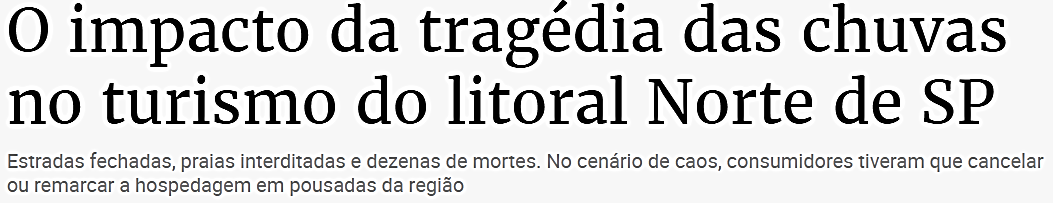
\includegraphics[width=1.78261in,height=0.90032in]{media/image6.png}

Todos os planetas possuem dois movimentos: rotação (em torno do seu
próprio eixo) e translação (em torno do sol). Vale ressaltar que
satélites, como a lua, também se movimentam. A lua gira em torno de si
mesma (rotação) e em torno da Terra (revolução), em conjunto esses
movimentos dão origem as fases lunares. Especificamente sobre a Terra, a
rotação dura cerca de 24 horas, ao longo desse período uma parte no
planeta fica iluminada pelo sol, enquanto a outra fica escura,
originando assim os dias e as noites. Já a translação dura cerca de 365
dias, 5 horas, 48 minutos e 48 segundos, esse movimento está ligado ao
fenômeno das estações do ano.

Além dessas características, a terra tem um outro atributo que a torna
especial dentre os planetas do nosso sistema solar: a vida. A
temperatura amena, a atmosfera contendo oxigênio e a presença da água em
forma líquida são fatores que favoreceram o aparecimento da vida no
planeta. Os organismos vivos habitam a camada mais superficial da Terra,
chamada de crosta, formada por rochas, minerais e solo. Entretanto,
nessa região enfrentamos diversos problemas ambientais, como
desmatamento, poluição das águas e do ar, degradação do solo e muitos
outros. Todos esses em conjunto, tem levado a extinção de diversas
espécies. Além da crosta, a terra é formada também pelo manto superior e
inferior, camadas intermediárias e pelo núcleo, camada mais interna.}

\colorsec{Atividades}

\num{1}  Trienalmente, a União Astronômica Internacional se reúne para tomada
  de decisões sobre astronomia e todas as suas vertentes. Em 2006,
  formularam uma nova classificação para os corpos celestes do Sistema
  Solar, na qual Plutão deixou de ser considerado planeta. Explique a
  principal característica que levou o grupo a tomar essa decisão.

\linhas{2}

\coment{Para que um corpo celeste seja considerado planeta ele deve ser capaz de
apresentar uma órbita própria, e Plutão não atendia a esse requisito,
tendo sua órbita dependente de outros corpos celestes.}

\num{2} Os planetas do Sistema Solar podem ser classificados de acordo com sua
  composição, sabendo disso, marque V para as afirmações verdadeiras e F
  para as falsas:

\begin{boxlist}
\item Marte é um planeta Joviano devido a sua composição rochosa. \alternativa{(F)
Marte é um planeta telúrico devido a sua composição rochosa}

\item Saturno é um planeta composto por hidrogênio, hélio e metano,
portanto, pode-se afirmar que é um planeta gasoso. \alternativa{(V)}

\item Terra é um planeta Joviano devido ao surgimento tardio de vida em
sua crosta. \alternativa{(F) A Terra é um planeta Telúrico pois apresenta crosta
rochosa}

\item Assim como Mercúrio, Vênus é um planeta Telúrico. \alternativa{(V)}
\end{boxlist}

\num{3}  Complete as lacunas a seguir.

\coment{Mercúrio}\preencher é um planeta rochoso, conhecido por ser
o mais próximo do sol e, portanto, o primeiro do nosso sistema solar. Em
contrapartida, \preencher é um planeta gasoso e o mais distante
do sol, devido a essa característica, suas temperaturas são muito
baixas, podendo alcançar -200°C. \coment{Netuno}

\num{4}  Em nosso sistema solar, existem cinco planetas classificados como anões. Cite o nome de cada um deles.

\linhas{1}

\coment{Plutão, Ceres, Haumea, Makemake, Eris.}

\num{5}  Sobre os movimentos do planeta Terra, marque R para características da rotação e T para características da translação.

\begin{boxlist}
\item Dura 24 horas. \alternativa{(R)}

\item Origina as estações do ano. \alternativa{(T)}

\item Dura 365 dias e alguns minutos, o que gera, após 4 anos, um ano
bissexto. \alternativa{(T)}

\item Origina os dias e as noites. \alternativa{(R)}
\end{boxlist}

\num{6}  O que é o Big Bang? Explique como e quando esse fenômeno ocorreu.

\linhas{3}

\coment{O Big Bang foi uma grande explosão gerada pelo acúmulo de energia e
calor em um ``átomo primordial'' extremamente denso. Após a explosão
toda a matéria entrou em expansão e assim se encontra até hoje.}

\num{7}  Uma teoria, já descartada, segundo a qual o Universo se contrairia até
  se reduzir a um único ponto, denso e quente, e então entraria em
  colapso -- quase como o inverso do Big Bang. Cientistas acreditavam
  que isso aconteceria porque a atração gravitacional poderia diminuir a
  velocidade de expansão das galáxias. Mas a hipótese foi derrubada em
  1998. ``Hoje sabemos que a densidade do Universo é baixa demais e que
  sua expansão não está desacelerando, e sim aumentando'', explica Raul
  Abramo, do Instituto de Física da USP.

\fonte{Referência:
https://super.abril.com.br/mundo-estranho/o-que-e-a-teoria-do-big-crunch/. Acesso em 24/02/2023.}

A qual teoria o texto se refere?

\linhas{1}

\coment{Big Crunch}

\num{8} Sobre a estrutura interna da Terra, indique a nomenclatura de cada camada ilustrada abaixo corretamente:


%\textless{}Diagramação, por favor, baixar imagem presente no link:
%\url{https://br.freepik.com/vetores-gratis/camadas-da-terra-desenhadas-a-mao-ilustradas_18774832.htm\#query=camadas\%20da\%20terra\&position=44\&from_view=search\&track=ais}
%\textgreater{} 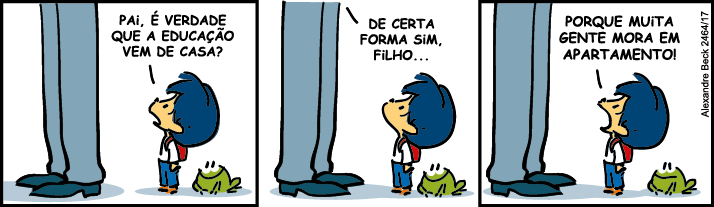
\includegraphics[width=2.58803in,height=2.75652in]{media/image7.png}

\linhas{1}

\coment{De cima para baixo são: crosta, manto superior, manto inferior e núcleo.}

\num{9}  Lúcia e sua irmã mais nova, Lara, gostam de observar o céu pela noite.
  Em uma das observações Lara notou que a Lua havia mudado e questionou
  sua irmã mais velha: ``Por que conseguimos ver a lua de várias
  formas?''. Como você aconselharia Lúcia a explicar esse fenômeno para
  sua irmã?

\linhas{2}

\coment{Lúcia deve explicar que vemos a lua em diferentes fases devido a
luminosidade que recebe do Sol a medida que ela se desloca ao redor da
Terra.}

\num{10}  Dentre todos os planetas do nosso Sistema Solar, pode-se dizer que a
  Terra tem uma característica especial, tendo em vista a vida que
  abriga. Descreva quais fatores tornaram possível a formação da vida na
  Terra.

\linhas{3}

\coment{A Terra encontra-se em uma região chamada de habitável em nosso sistema
solar. Ou seja, ela recebe radiação solar suficiente para manter a
temperatura estável, permitindo a existência de água na forma líquida,
essencial para a vida.}

\colorsec{SEÇÃO TREINO}

\num{1} Observe a imagem a seguir, e com base nos seus conhecimentos identifique quais são os planetas rochosos presentes no nosso sistema solar:

%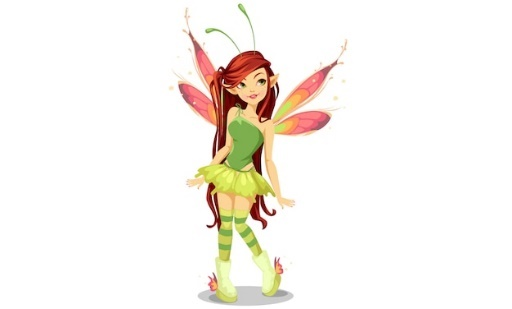
\includegraphics[width=2.89583in,height=2.89583in]{media/image8.jpeg}

%Esquema do Nosso Sistema Solar. Disponível em:
%\url{https://br.freepik.com/vetores-gratis/esquema-do-sistema-solar-colorido-com-design-plano_2826128.htm?query=planetas\%20do\%20sistema\%20solar\#from_view=detail_alsolike}.
%Acesso em 24 de fevereiro de 2023.

\begin{escolha}
\item
  Mercúrio, Vênus, Terra e Júpiter
\item
  Netuno, Saturno, Terra e Urano
\item
  Mercúrio, Vênus, Terra e Marte
\item
  Saturno, Urano, Netuno e Plutão
\end{escolha}

\coment{Fácil - Habilidade BNCC: (EF09CI14) Descrever a composição e a estrutura
do Sistema Solar (Sol, planetas rochosos, planetas gigantes gasosos e
corpos menores), assim como a localização do Sistema Solar na nossa
Galáxia (a Via Láctea) e dela no Universo (apenas uma galáxia dentre
bilhões).

a) INCORRETA, pois Júpiter é um planeta gasoso.

b) INCORRETA, pois dos planetas citadas apenas a Terra faz parte dos
  planetas rochosos.

c) CORRETA, de fato os planetas citados fazem parte dos planetas
  rochosos.

d) INCORRETA, os planetas citados são os planetas gasosos.}

\num{2} Observe a imagem a seguir:

%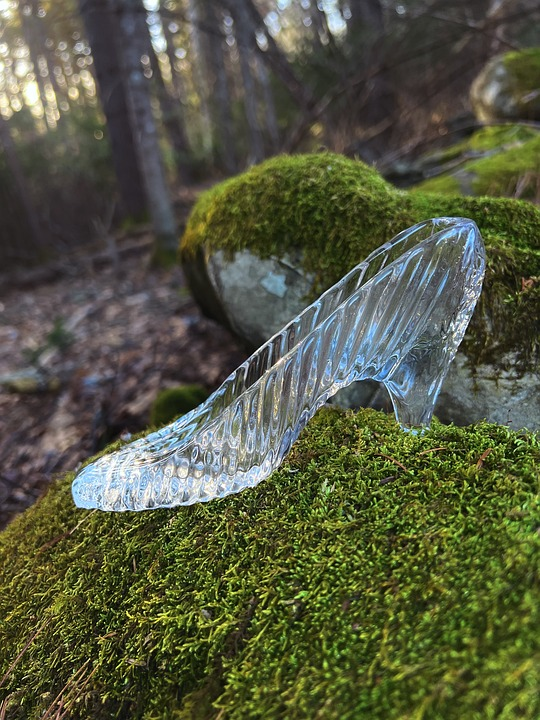
\includegraphics[width=2.77865in,height=2.63750in]{media/image9.jpeg}

%Novas fotos do James Webb podem revelar segredos sobre o nascimento de estrelas. CNN Brasil. 12/09/2022. Disponível em: \url{https://www.cnnbrasil.com.br/tecnologia/novas-fotos-do-james-webb-podem-revelar-segredos-sobre-o-nascimento-de-estrelas/}. Acesso: 20 de fevereiro de 2023.

A imagem tirada pelo Telescópio Espacial James Webb (NASA) mostra o
interior de uma nebulosa, onde nascem as estrelas. A partir dos seus
conhecimentos justifique como é possível identificar o nascimento de
estrelas

\begin{escolha}
\item
  Através da observação de elementos pesados e matéria escura
\item
  Através da identificação de ferro na superfície da estrela
\item
  Através da presença de grande quantidade de energia, gás e poeira
  cósmica
\item
  Através da observação da Gigante vermelha em torno de uma nuvem de
  poeira
\end{escolha}

\coment{Média -- Habilidade BNCC: (EF09CI17) Analisar o ciclo evolutivo do Sol
(nascimento, vida e morte) baseado no conhecimento das etapas de
evolução de estrelas de diferentes dimensões e os efeitos desse processo
no nosso planeta.

a) INCORRETA, pois quando há presença de elementos pesados é
  característico do fim da vida da estrela

b) INCORRETA, pois a presença de ferro na superfície e interior de uma
  estrela é característica do fim da vida da estrela

c) CORRETA, pois de fato a presença de grande quantidade de energia,
  poeira cósmica e gás são os elementos presentes no início da vida de
  uma estrela

d) INCORRETA, pois a presença de uma Gigante vermelha significa que a
  estrela está em crescimento.}

\num{3}

\begin{quote}
Cientistas da Universidade da Califórnia-Riverside
(UCR) \textbf{simularam sistemas alternativos}~do nosso Sistema Solar,
descobrindo que se a órbita de Júpiter fosse mais achatada --- ou
"excêntrica" --- ela causaria grandes mudanças na órbita
do nosso
planeta. Se a órbita de Júpiter se tornasse mais excêntrica, a equipe
descobriu que a órbita da Terra seria empurrada para se tornar mais
excêntrica também. Isso significa que às vezes a Terra estaria ainda
mais perto do Sol do que já está. A equipe acha que seus resultados
podem ajudar os astrônomos a determinar quais planetas fora do Sistema
Solar -- exoplanetas -- poderiam ser habitáveis.

\fonte{Mudança na órbita de Júpiter poderia tornar a Terra ainda mais favorável
à vida. Sputinik Brasil. 14/09/2022. Disponível em:
https://sputniknewsbrasil.com.br/20220914/mudanca-na-orbita-de-jupiter-poderia-tornar-a-terra-ainda-mais-favoravel-a-vida-24777610.html.
Acessado em: 20 de fevereiro de 2023.}
\end{quote}

Identifique dentre as alternativas aquela que descreve um importante
fator para a habitabilidade em um planeta:

\begin{escolha}
\item
  A distância de um planeta e sua estrela deve possibilitar temperaturas
  amenas e com baixas variações para que seja possível a existência de
  água líquida
\item
  A órbita dos satélites naturais ao redor desse planeta deve ser a
  mesma órbita do planeta para que haja formação de água líquida
\item
  O aumento da distância percorrida pelo planeta deve proporcionar
  aumento das regiões polares evitando aquecimento do planeta
\item
  A inclinação do planeta deve permitir a radiação emitida pela sua
  estrela seja a menor possível pois radiação é nociva
\end{escolha}

\coment{Difícil- Habilidade BNCC: (EF09CI16) Selecionar argumentos sobre a
viabilidade da sobrevivência humana fora da Terra, com base nas
condições necessárias à vida, nas características dos planetas e nas
distâncias e nos tempos envolvidos em viagens interplanetárias e
interestelares.

a) CORRETA, pois de fato a distância em que o planeta se encontra de sua
  estrela é o principal ponto que os cientistas observam para
  identificar planetas em zonas habitáveis no espaço.

b) INCORRETA, pois a órbita dos satélites naturais de um planeta não
  necessariamente se relaciona coma formação de água naquele planeta

c) INCORRETA, pois ao aumentar a distância entre um planeta e sua estrela
  a quantidade de radiação e calor podem levar o planeta a super
  aquecer, o que não favorece o surgimento da vida como conhecemos

d) INCORRETA, pois apesar da inclinação do planeta ser um ponto
  extremamente relevante, a radiação que um planeta deve receber deve
  ser proporcional a sua posição e tamanho, para que hajam temperaturas
  amenas para o surgimento da vida}

\chapter{QUESTÕES SIMULADO 1}

\num{1}
  \begin{quote}
  Os advogados de defesa de Willian da Silva Alves utilizaram leis da
  física para conseguir, na segunda-feira
  (23), a
  liberdade provisória do jovem, de 19 anos. Ele foi
  preso suspeito
  de assaltar um
  comércio em Cocal,
  267 km ao Norte
  de Teresina,
  após suposto reconhecimento da vítima. Conforme a defesa de Willian,
  ele estava almoçando na casa da sogra, na Zona Rural de Cocal, no
  momento em que o roubo, no Centro do município, aconteceu. Os
  advogados do jovem, Batista Filho Júnior e Bruno Portela, basearam a
  defesa no \textbf{princípio da impenetrabilidade da matéria}.

\fonte{G1 Notícias Piauí, 24/01/2023. Disponível em:
https://g1.globo.com/pi/piaui/noticia/2023/01/24/defesa-usa-formulas-fisicas-para-conseguir-liberdade-provisoria-de-jovem-no-pi-impossivel-estar-em-dois-locais-ao-mesmo-tempo.ghtml.
Acesso em: 24 de fevereiro de 2023.}
\end{quote}

Identifique dentre as alternativas aquela explica corretamente o
conceito de impenetrabilidade

\begin{escolha}
\item
  Qualquer matéria pode ser dividida em pedaços menores que os iniciais
\item
  Um corpo tende a permanecer em seu estado natural até que outra força
  haja sobre ele
\item
  Duas porções de matéria não podem ocupar o mesmo espaço ao mesmo tempo
\item
  Toda matéria ocupa lugar no espaço
\end{escolha}

\coment{Média -- Habilidade BNCC: (EF09CI01) Investigar as mudanças de estado
físico da matéria e explicar essas transformações com base no modelo de
constituição submicroscópica.

a)  INCORRETA, pois traz o conceito da propriedade divisibilidade

b)  INCORRETA, pois traz o conceito da propriedade inércia

c)  CORRETA, pois traz exatamente o conceito de impenetrabilidade

d)  INCORRETA, pois traz o conceito da propriedade extensão.}

\num{2}
\begin{quote}
Segundo dados do Instituto Nacional de Câncer (INCA), são esperados
60 mil novos casos de câncer de mama no Brasil em 2018, os números
crescem a cada ano e a neoplasia continua sendo a segunda maior causa
de morte entre as mulheres brasileiras. Fatores genéticos correspondem
à 12\% dos casos de câncer de mama e aumentam em 80\% as chances do
desenvolvimento deste tipo de câncer.

\fonte{HEREDITARIEDADE AUMENTA EM 80\% AS CHANCES DE SE DESENVOLVER CÂNCER DE
MAMA. Hospital Oswaldo Cruz, 28/09/2018. Disponível em:
https://www.hospitaloswaldocruz.org.br/imprensa/noticias/hereditariedade-aumenta-em-80-as-chances-de-se-desenvolver-cancer-de-mama/.
Acesso em: 24 de fevereiro de 2023.}
\end{quote}

Uma doença hereditária é aquela que passa de pai pra filho no decorrer
das gerações. Identifique a alternativa que explica geneticamente como a
hereditariedade influência no aparecimento do câncer

\begin{enumerate}
\item
  Os filhos herdam 100\% seu material genético dos genitores através das
  células germinativas, recebendo os genes com mutações cancerígenas
\item
  Os filhos herdam 50\% do material genético dos genitores e os outros
  50\% são adquiridos no decorrer da vida, onde pode ocorrer mutações
  cancerígenas
\item
  O câncer de mama está presente apenas no DNA de mulheres sendo herdado
  100\% do DNA das mães
\item
  Alterações genéticas cancerígenas como o câncer de mama são adquiridas
  na hora do parto, sendo herdadas exclusivamente dos pais.
\end{enumerate}

\coment{Difícil -- Habilidade BNCC: (EF09CI08) Associar os gametas à transmissão
das características hereditárias, estabelecendo relações entre
ancestrais e descendentes.


a)  CORRETA, pois os fatores hereditários são herdados dos genitores
  através das células germinativas no ato da fecundação.

b)  INCORRETA, pois os filhos herdam 100\% do seu material genético dos
  genitores sendo 50\% herdado da mãe e os outros 50\% herdados do pai.

c)  INCORRETA, pois apesar do câncer de mama ser mais agressivo em
  mulheres ele também ocorre em homens.

d)  INCORRETA, pois alterações genéticas não são adquiridas na hora do
  parto já que se trata de alterações moleculares envolvendo a formação
  de indivíduos.}

\num{3}
\begin{quote}
  Com um tamanho pouco superior ao da nossa lua, é o planeta mais
  pequeno do sistema solar e o mais próximo do Sol. Trata-se do menor
  dos planetas rochosos dos planetas do sistema solar e, tal como a Lua,
  apresenta uma superfície repleta de crateras, em parte devido à
  finíssima e quase ausente atmosfera (exosfera) que o rodeia. Com uma
  velocidade de 170.5030 quilómetros por hora, trata-se também do
  planeta que viaja mais depressa através do espaço -- daí o seu nome --
  já que a velocidade de um planeta aumenta em função da sua proximidade
  da estrela que orbita.

\fonte{Assim são os 8 planetas do sistema solar. National Geographic,
03/02/2023. Disponível
em:https://nationalgeographic.pt/ciencia/grandes-reportagens/3494-assim-sao-os-8-planetas-do-sistema-solar.
Acesso em: 22 de fevereiro de 2023.}
\end{quote}

A partir da leitura do texto e com base nos seus conhecimentos,
identifique o planeta ao qual o texto se refere

\begin{escolha}
\item
  Mercúrio
\item
  Vênus
\item
  Plutão
\item
  Saturno
\end{escolha}

\coment{Fácil -- Habilidade BNCC: (EF09CI14) Descrever a composição e a
estrutura do Sistema Solar (Sol, planetas rochosos, planetas gigantes
gasosos e corpos menores), assim como a localização do Sistema Solar na
nossa Galáxia (a Via Láctea) e dela no Universo (apenas uma galáxia
dentre bilhões).


a)  CORRETA, pois o menor planeta e mais próximo do Sol é Mercúrio.

b)  INCORRETA, pois Vênus é o segundo planeta em proximidade ao Sol e seu
  tamanho é parecido com o da Terra.

c)  INCORRETA, pois Plutão é um planeta anão e se localiza extremamente
  distante do Sol.

d)  INCORRETA, pois Netuno é o planeta mais distante do sol e sua
  superfície é formada por gases.}

\chapter{SIMULADO 2}

\num{1}
  No século 18 um químico francês chamado Lavoisier realizava
  experimentos de combustão e calcinação utilizando balanças para medir
  seus produtos e reagentes afim de garantir bons dados quantitativos. A
  partir das medições feitas por Lavoisier nesses experimentos ele
  postulou o que chamamos de Lei de Lavoisier.

\fonte{Texto autoral.}

Identifique dentre as alternativas aquela que apresenta um outro nome
para a Lei de Lavoisier e sua definição

\begin{escolha}
\item
  Lei da Inércia. Toda matéria deve permanecer no estado em que se
  encontra até que uma força haja sobre ela
\item
  Lei das proporções constantes. Toda substância apresenta uma proporção
  constante em sua composição
\item
  Lei de Gay-Lussac. Em pressão e temperatura constantes os volumes dos
  gases de uma reação tem entre si uma relação de números inteiros.
\item
  Lei de conservação das massas. Em um sistema fechado a massa total dos
  reagentes é igual a massa total dos produtos.
\end{escolha}

\coment{Fácil -- Habilidade BNCC: (EF09CI02) Comparar quantidades de reagentes e
produtos envolvidos em transformações químicas, estabelecendo a
proporção entre as suas massas.


a)  INCORRETA, pois a Inércia também conhecida como primeira lei de Newton
  não diz respeito a conservação das massas em uma reação.

b)  INCORRETA, pois a lei da proporção fala da composição das substâncias
  envolvidas em uma reação.

c)  INCORRETA, a lei de Gay-Lussac, além de não ser proposta por
  Lavoisier, trata das condições que influenciam uma reação como pressão
  e temperatura.

d)  CORRETA, pois a Lei de Lavoisier é justamente a Lei de conservação das
  massas, onde a massa dos reagentes deve ser igual a massa do produto.}

\num{2}
  Um fungo aquático que já levou à extinção diversas espécies de
  anfíbios que têm parte ou todo o ciclo de vida na água ameaça também
  os sapos terrestres. Um grupo de pesquisadores apoiado pela FAPESP
  constatou na Mata Atlântica uma mortandade sem precedentes de sapinhos
  que se desenvolvem longe do ambiente aquático. Os anfíbios estavam
  infectados com altas cargas do fungo quitrídio (\emph{Batrachochytrium
  dendrobatidis}), causador da quitridiomicose.

\fonte{Agência Fapesp, 16/09/2021. Disponível em:
https://agencia.fapesp.br/fungo-aquatico-que-ja-extinguiu-diversas-especies-de-anfibios-ameaca-agora-sapos-terrestres-diz-estudo/36843/.
Acesso em: 23 de fevereiro de 2023.}

Indique a alternativa que mostra uma possível consequência do declínio
da população de anfíbios:

\begin{escolha}
\item Além da perda de biodiversidade, as relações dentro do ecossistema
são afetadas, tendo em vista que anfíbios possuem diversas funções
ecológicas, como o controle de insetos transmissores de doenças.

\item A rápida dispersão do fungo causador da quitridiomicose, impede a
evolução de outras espécies que habitam o ecossistema, tendo em vista a
necessidade de investir energia apenas na fuga.

\item As populações de anfíbios que passam a maior parte do ciclo na terra
não são afetadas pelo fungo, entretanto, são obrigadas a mudar sua
reprodução, que depende da água, para evitar os fungos.

\item A alta pressão exercida pelos fungos na população de anfíbios, fará
com que sapos, rãs e pererecas se modifiquem para adquirir resistência
ao patógeno.
\end{escolha}

\coment{Média -- Habilidade BNCC (EF09CI11) Discutir a evolução e a diversidade
das espécies com base na atuação da seleção natural sobre as variantes
de uma mesma espécie, resultantes de processo reprodutivo.

a) CORRETA, pois ao dizimar populações, o fungo reduz a riqueza de
espécies de anfíbios, ou seja, afeta a biodiversidade da área. Além de
impactar o equilíbrio do ecossistema pois anfíbios servem de alimento
para outros animais, comem artrópodes e controlam comunidades de
invertebrados.

b) INCORRETA, pois a evolução é um processo constante e atemporal,
portanto, acontecerá independente das imprevisibilidades existentes
dentro de um ecossistema, como a endemia citada.

c) INCORRETA, pois o texto base comenta que os fungos começam a ameaçar
também sapos que habitam o ambiente terrestre, portanto, estes
organismos serão afetados independente do seu modo de reprodução.

d) INCORRETA, pois a alternativa faz alusão a teoria evolucionista
pensada por Lamarck, que não é adotada atualmente e afirma que os seres
vivos se modificam para sobreviver no ambiente.}

\num{3}
\begin{quote}
Um trabalho gigantesco, que envolveu centenas de cientistas, 5 anos
de investigações e telescópios espalhados por oito lugares diferentes
do planeta foi capaz de captar as primeiras imagens do Sagittarius A*,
um buraco negro localizado no centro da Via Láctea, a galáxia em que
se encontra o nosso Sistema Solar. O objeto tem impressionantes quatro
milhões de vezes a massa do Sol e foi retratado pela primeira vez
graças a um esforço colaborativo de centenas de cientistas, reunidos
no projeto~\emph{Event Horizon Telescope}~(EHT).

\fonte{BBC News Brasil, 13/05/2022. Disponível em:
https://www.bbc.com/portuguese/internacional-61440848. Acesso em:
24 de fevereiro de 2023.}
\end{quote}

Buracos negros causam fascínio por conta da sua magnitude e potencial
perigo. Quais seriam as possíveis consequências para o nosso planeta
caso nossa galáxia se chocasse com outra?

\begin{escolha}
\item
  Toda a matéria da Terra se separaria em partículas minúsculas, além da
  noção de tempo que dentro de um buraco negro é quase nula.
\item
  Por ser muito pequena a Terra passaria ilesa pelas proximidades de um
  buraco negro sem ser engolida.
\item
  A força gravitacional da Terra deformaria o buraco negro, mas mesmo
  assim ela seria absorvida e sua matéria seria incorporada pelo próprio
  buraco.
\item
  A força gravitacional do buraco negro empurraria a Terra de tal forma
  que o planeta se chocaria em outro corpo celeste com muita velocidade
\end{escolha}

\coment{Difícil -- Habilidade BNCC: (EF09CI17) Analisar o ciclo evolutivo do Sol
(nascimento, vida e morte) baseado no conhecimento das etapas de
evolução de estrelas de diferentes dimensões e os efeitos desse processo
no nosso planeta.


a)  CORRETA, pois a força gravitacional de um buraco negro atrairia a
  Terra com tanta intensidade que toda a matéria da Terra se separaria
  em pequenas partículas e o tempo passaria extremamente lento.

b)  INCORRETA, pois mesmo sendo bastante pequena em comparação a um buraco
  negro, a Terra seria engolida e destruída por ele.

c)  INCORRETA, pois no encontro de duas galáxias as condições seriam
  catastróficas e o buraco negro formado pelo encontro do centro dessas
  galáxias seria gigantesco, dessa forma a força gravitacional da Terra
  seria imperceptível.

d) INCORRETA, pois a força gravitacional do buraco negro tente a puxar os
  corpos para si, engolindo a Terra, mesmo com a existência do efeito
  estilingue que acontece na borda de um buraco negro.}

\chapter{SIMULADO 3}

\num{1}
\begin{quote}
  O nome vem do grego~\emph{atomos}, que significa indivisível. Mas os
  físicos já sabem hoje que os átomos não são sólidos como pequenas
  esferas, e sim uma espécie de sistema planetário elétrico minúsculo.
  Eles são constituídos por três partes principais: prótons, nêutrons e
  elétrons. Pense nos prótons e nos nêutrons unidos no centro formando o
  ``sol'', ou núcleo. E os elétrons orbitando esse núcleo, como
  planetas. Elétrons se movimentam de um átomo a outro de um fio de
  cobre, carregando consigo a carga pela extensão do fio.

\fonte{Modificado de BBC News Brasil, 21/01/2016. Disponível em:
https://www.bbc.com/portuguese/noticias/2016/01/160113\_vert\_earth\_como\_sabemos\_que\_atomos\_existem\_rw.
Acesso em: 24 de fevereiro de 2023.}
\end{quote}

Sabendo que os elétrons podem se movimentar independentes dos seus
átomos, escolha a alternativa que justifica um possível experimento para
provar essa movimentação dos elétrons.

\begin{escolha}
\item
  Submeter os elétrons a um processo de liofilização para observar se
  havia uma repulsão de cargas
\item
  Colocar os elétrons sobre feixes de luz super potentes para que fosse
  possível observar sua movimentação
\item
  Ionizar os átomos doando cargas negativas para repelirem os elétrons e
  observar sua movimentação
\item
  Centrifugar os elétrons, já que nesse processo seriam doadas cargas
  positivas e observar se há movimentação
\end{escolha}

\coment{Difícil -- Habilidade BNCC: (EF09CI03) Identificar modelos que descrevem
a estrutura da matéria (constituição do átomo e composição de moléculas
simples) e reconhecer sua evolução histórica.


a)  INCORRETA, o processo de liofilização consiste na retirada de água de
  uma substância, elétrons não possuem água.

b)  INCORRETA, os elétrons são tão pequenos que não são captados pelas
  ondas luminosas e dessa forma são invisíveis para a luz.

c)  CORRETA, a ionização, ou seja, doação de cargas faz com que os
  elétrons se excitem e se movimentem pelos átomos.

d)  INCORRETA, o processo de centrifugação consiste em agitar substâncias
  afim de apressar o processo de decantação, o que não faz sentido para
  elétrons.}

\num{2}
\begin{quote}
Com o objetivo de preservar a biodiversidade e garantir o menor
impacto ambiental possível em projetos de infraestrutura de
transportes, Ministério dos Transportes e Instituto Brasileiro do Meio
Ambiente e dos Recursos Naturais Renováveis (Ibama) decidiram
fortalecer a parceria entre os dois órgãos do Governo Federal. Nesta
quinta-feira (23), o ministro dos Transportes, Renan Filho, e o
presidente do Instituto Brasileiro do Meio Ambiente e dos Recursos
Naturais Renováveis (Ibama), Rodrigo Agostinho, reuniram-se para
tratar de projetos em rodovias onde há grande riqueza de fauna e
flora, incluindo espécies ameaçadas de extinção, os quais necessitam
da junção de esforços visando à preservação ambiental.

\fonte{Governo Federal do Brasil. 24/02/2023. Disponível em:
https://www.gov.br/infraestrutura/pt-br/assuntos/noticias/2023/02/parceria-vai-fortalecer-preservacao-de-fauna-e-flora-nas-imediacoes-de-rodovias.
Acesso em: 25 de fevereiro de 2023.}
\end{quote}

Uma possível medida que visa conciliar o avanço da infraestrutura do
País com a proteção ambiental é:

\begin{escolha}
\item
  Construção de corredores ecológicos entre as vias para que os animais
  possam atravessar entre os ambientes em segurança.
\item
  Investir na locomoção por vias aquáticas e aéreas para evitar a
  construção de pistas e degradação ambiental.
\item
  Isolar cidades e comunidades que vivem em regiões de alta
  biodiversidade evitando a degradação ambiental
\item
  Cobrar taxas de circulação para quem for circular por vias que se
  localizem em regiões onde há presença de animais silvestres
\end{escolha}

\coment{Média -- Habilidade BNCC: (EF09CI12) Justificar a importância das
unidades de conservação para a preservação da biodiversidade e do
patrimônio nacional, considerando os diferentes tipos de unidades
(parques, reservas e florestas nacionais), as populações humanas e as
atividades a eles relacionados.


a)  CORRETA, pois a construção de corredores ecológicos se feita sob um
  estudo e com planejamento visa preservar a possibilidade de locomoção
  de animais, bem como a passagem de rodovias para a circulação de seres
  humanos.

b)  INCORRETA, pois a locomoção por vias aquáticas e aéreas também geram
  impactos ambientais e colocam em risco a vida de animais, além de
  serem menos vantajosas para viagens dentro do País.

c)  INCORRETA, pois isolar cidades e comunidades limitaria o acesso dos
  moradores a educação, saúde e até alimentação.

d)  INCORRETA, pois cobrar taxas de circulação não garante que vá haver
  manutenção e proteção da biodiversidade presente no local.}

\num{3}
  Na antiguidade o eclipse solar era considerado algo místico. Na Grécia
  antiga por exemplo, o eclipse solar era sinônimo da ira dos Deuses.
  Com o avanço da ciência foi possível identificar o que de fato é um
  eclipse solar e como ele acontece.

\fonte{Texto autoral.}

Identifique a partir das alternativas a seguir aquela que explica
corretamente como ocorre um eclipse solar.

\begin{escolha}
\item
  Um eclipse solar ocorre quando o Sol se posiciona entra a Terra e a
  Lua.
\item
  Um eclipse solar ocorre quando a Lua se posiciona entra a Terra e o
  Sol.
\item
  Um eclipse solar ocorre quando Marte e a Lua passam entre o Sol e a
  Terra.
\item
  Um eclipse solar ocorre quando a Terra fica entre o Sol e a Lua.
\end{escolha}

\coment{Fácil -- Habilidade BNCC: (EF09CI14) Descrever a composição e a
estrutura do Sistema Solar (Sol, planetas rochosos, planetas gigantes
gasosos e corpos menores), assim como a localização do Sistema Solar na
nossa Galáxia (a Via Láctea) e dela no Universo (apenas uma galáxia
dentre bilhões).


a)  INCORRETA, pois não há possibilidades do Sol fica entre a Terra e a
  Lua por conta dos seus tamanhos, distâncias e órbitas

b)  CORRETA, pois em um eclipse solar a Lua fica entre o Sol e a Terra
  evitando que a luz solar chegue completamente em alguns pontos da
  Terra.

c)  INCORRETA, pois não há possibilidades de Marte passar entre o Sol e a
  Terra já que Marte se encontra mais distante do Sol que a própria
  Terra.

d)  INCORRETA, pois quando a Terra se encontra entre a Lua e o Sol temos
  um eclipse lunar.}

\chapter{SIMULADO 4}

\num{1}
\begin{quote}
  A fusão nuclear é um tipo de energia nuclear diferente do processo
  de fissão nuclear que é usado desde 1950 nos reatores de energia
  atômica. Na fusão, a energia é gerada a partir da união de átomos,
  enquanto na fissão a energia é gerada pela divisão de átomos. A fusão
  é o processo que ocorre no Sol continuamente, responsável pelo seu
  calor e sua luz.

\fonte{BBC News Brasil, 15/11/2019. Disponível em:
https://www.bbc.com/portuguese/geral-50422745. Acesso em: 25 de
fevereiro de 2023.}
\end{quote}

Com base nos matérias e no processo utilizados para a produção de
energia a partir da fusão nuclear podemos afirmar que:

\begin{escolha}
\item
  Trata-se da união de elétrons a partir de liberação uma grande
  quantidade de energia
\item
  Trata-se da união de dois núcleos, para formar um mais denso sendo
  necessária grande quantidade de energia e pressão
\item
  Trata-se de um processo prejudicial que gera lixo radioativo pois
  utiliza compostos químicos tóxicos.
\item
  Trata-se de um processo barato e simples já que se trata de uma cópia
  de um processo que ocorre naturalmente no Sol
\end{escolha}

\coment{Médio -- Habilidade BNCC: (EF09CI03) Identificar modelos que descrevem a
estrutura da matéria (constituição do átomo e composição de moléculas
simples) e reconhecer sua evolução histórica.


a)  INCORRETA, pois a fusão não se refere a união de elétrons e sim a
  união de núcleos atômicos.

b)  CORRETA, pois a fusão é justamente a união de núcleos atômicos e para
  manipular esses núcleos são necessárias grande quantidades de energia
  e pressão

c)  INCORRETA, pois utilizando basicamente hidrogênio a fusão não libera
  resíduos radioativos

d)  INCORRETA, pois não se trata de um processo barato, pelo contrário, a
  fusão nuclear é caríssima pelas condições que necessita para acontecer.}

\num{2}
\begin{quote}
  De acordo com sua teoria, há uma luta pela sobrevivência na
  natureza, mas aquele que sobrevive não é necessariamente o mais forte
  e, sim, o que melhor se adapta às condições do ambiente em que vive.
  No ambiente árido, as tartarugas de pescoço longo alcançavam os
  arbustos para se alimentar. Enquanto aquelas que viviam em local
  úmido, podiam comer grama e se proteger dos predadores graças ao
  pescoço curto e à carapaça arredondada.

\fonte{BBC News Brasil, 22/11/2023. Disponível em:
https://www.bbc.com/portuguese/geral-50525124. Acesso em: 23 de
fevereiro de 2023.}
\end{quote}

A partir do texto e de seus conhecimentos, identifique a alternativa de
apresenta o conceito e o cientista por trás do conceito descrito

\begin{escolha}
\item
  Lei do uso e desuso, Darwin
\item
  Lei dos caracteres adquiridos, Lamarck
\item
  Lei da seleção natural, Darwin
\item
  Lei da seleção natural, Lamarck
\end{escolha}

\coment{Fácil -- Habilidade BNCC: (EF09CI10) Comparar as ideias evolucionistas
de Lamarck e Darwin apresentadas em textos científicos e históricos,
identificando semelhanças e diferenças entre essas ideias e sua
importância para explicar a diversidade biológica.


a)  INCORRETA, pois a lei do uso e desuso fala que ao usar mais uma
  estrutura ela vai se tornar melhor e conferir vantagens no meio
  ambiente em que a espécie vive, além de não ter sido descrita por
  Darwin

b)  INCORRETA, pois a lei dos caracteres adquiridos diz que a espécie se
  adequa ao meio em que vive e passa isso para as gerações seguintes

c)  CORRETA, pois o texto trás exatamente um exemplo de como a seleção
  natural atua sobre as espécies

d)  INCORRETA, pois a lei da seleção natural não foi descrita por Lamarck.}

\num{3}
  \begin{quote}
  O projeto \emph{Mars One}, da Holanda, foi lançado em 2012 e foram
  escolhidas 40 pessoas - entre 200 mil candidatos. O projeto é
  financiado por um programa estilo "reality show" - que pretende
  treinar as pessoas para uma vida no planeta vermelho. Para muitos, a
  ideia é uma grande brincadeira, mas mostra que já existe gente
  interessada no assunto. A empresa \emph{SpaceX} também tem projetos
  para colonizar Marte - mas com um pouco mais seriedade. A empresa
  imagina um veículo gigante chamado \emph{Mars Colonial Transporter},
  que seria usado para várias viagens entre a Terra e Marte.

\fonte{BBC News Brasil, 11/10/2014. Disponível em:
https://www.bbc.com/portuguese/noticias/2014/10/141010\_vert\_fut\_colonia\_espaco\_dg.
Acesso em: 25 de fevereiro de 2023.}
\end{quote}

Imaginando que a colonização espacial seja uma realidade próxima, quais
possíveis consequências para o corpo de seres humanos nascidos no
espaço:

\begin{escolha}
\item
  Os corpos se tornam mais altos devido à ausência de gravidade e a
  diminuição do volume de sangue já que há menos esforço para o coração.
\item
  Pelo maior contato com a radiação os seres humanos seriam mais
  tolerantes a desenvolver câncer
\item
  Haveria o aumento da massa muscular e óssea provocadas pela
  microgravidade espacial, porém uma diminuição na altura
\item
  Melhora nas condições da visão devido ao controle de exposição a luz,
  acompanhadas de insônia pela diferença no fuso
\end{escolha}

\coment{Difícil -- Habilidade BNCC: (EF09CI16) Selecionar argumentos sobre a
viabilidade da sobrevivência humana fora da Terra, com base nas
condições necessárias à vida, nas características dos planetas e nas
distâncias e nos tempos envolvidos em viagens interplanetárias e
interestelares.


a)  CORRETA, pois a baixa gravidade exerceria menos pressão na coluna, o
  que tornaria as pessoas um pouco mais altas, e também a diminuição no
  volume do sangue que fluiria com mais facilidade pelo corpo já que não
  tem gravidade puxando para baixo

b)  INCORRETA, pois aconteceria justamente o contrário, pelo maior contato
  com radiação os seres humanos estariam mais suscetíveis a desenvolver
  tipos de câncer.

c)  INCORRETA, pois devido a movimentação com baixa gravidade ser
  diferente a massa muscular e óssea é diminuída, porém a altura aumenta

d)  INCORRETA, pois a visão tende a piorar no espaço primeiro pela
  diferença na incidência de luz, segundo pela mudança na pressão
  sofrida pelo olho.}


